\documentclass[HardwareDesign/HardwareDesign_main.tex]{subfiles}
\begin{document}
\section{Bolddispenser}
I det her afsnit vil der blive beskrevet de overvejelser, valg og udviklingsprocesser der skulle foretages under design af bolddispenser kredsløbet. Udvikling af komponenterne til bolddispenseren er baseret på prædefineret krav som kan læses under afsnittet \fullref{kravspec:sec:uc_4_refill_balls} i dokumentet \textbf{Kravspecifikation}. Afsnittet er strukturet efter blokbeskrivelsen af bolddispenseren under afsnittet \fullref{arch:sec:balldispenser_hardware_block_description} i \textbf{Akitektur} dokumentet.

\subsection{Bolddispenserens fysiske og mekaniske dele}
\subsubsection{Overvejelser}
Der findes mange mekaniske løsninger til dispensering af bolde. Den først metode som blev overvejet er den hvor to hjul sørger for at fremdrive bolden ud dispenseren, ligesom man gør med en tennis bolddispenser. Denne metode er dog mest brugt i tilfælde hvor der er behov for at få dispenseret bolden med en relativ høj hastighed. Fysisk fylder det også meget i forhold til nogle af de andre muligheder. Et andet løsning var at bruge den samme mekanisk system som bruges i typiske bordfodbolds borde. Fordelene er at man nemt kan finde en færdig design på nettet, og alle dele kan 3d printes. Ulempen er at der ikke bruges elektroniske aktuatorer.
Den tredje løsning som blev overvejet er en rotationsplatform mekanisme. Her udnytter man tyndekraften til at dispensere boldene. En cylinderformet beholder med et hul i bunden sider på den her roterende platform. For at dispensere boldene roteres platformen således at dens hul passer med hullet på bunden af cylinder-beholderen. Nå man så rotere igen, så bliver bolden i platformens hul dispenseret. Denne løsning er god fordi den bruger en aktuator til styring af dispensering, og den er simpel nok til at 3d printe. Ulempen er dog at platformen fylder meget.

\subsubsection{Valg}
Der valges platformløsningen da denne virker mest logisk. Fordi den mekaniske del er så simpel, så giver det rum til bedre udvikling af sensor og aktuator.

\subsubsection{Udviklingsproces}
Der købes ståltråde og gaffertape til udvikling af en pap prototype. Det er nødvendigt at lave en \textit{proof of concept} med en pap model før vi går i gang med alt andet. Der bruges tomme toiletpapirruller og køkkenruller til cylinder-beholderen. Under udvikling af beholderen blev jeg inspireret til at ændre mekanismen så der ikke var behov for en platform. I stedet for platformen skulle der være endnu en cylinderbeholder med et hul i siden. Denne mindre cylinder ville ligge under beholderen og holde boldene ind, ligesom platformen gjorde. For at dispensere bolde vil den rotere 180 grader rundt om beholderens højde-akse. Bolddispenseren bliver nu kompakt, mekanisk simpel, og nem at forbedre med aktuator og sensor. Boldispenserens fysisk konstruktion og dele kan ses på figur ????
(INDSÆT FIGUR!)
\subsection{Bolddispenserens Status LED's}
Disse LED'er står for at notificere brugeren om hvor vidt bolddispenseren har brug for flere bolde.
\subsubsection{Harware Design}
Der laves to transistor switch kredsløb til at styre de to LED'er. Disse bliver dimensioneret sådan så LED'er får ordenligt gas.
Kredsløbet er lavet vha. en bc517b
\subsection{Bolddispenserens Ball count sensor}
Denne sensor står for at notificere systemet om hvor vidt bolddispenseren har brug for flere bolde.
\subsubsection{Harware Design}
Det var klart i begyndelsen af design at dette skulle være en lyssensor. Boldene vejer for lidt til en pålidelig måling, og en kapacitans sensor er ikke praktisk i forhold til bolddispenserens fysiske dimensioner. Desuden er der meget mørkt i bolddispenseren så en lyssensor vil ikke blive forstyrret. I starten var der to lyssensorer der skulle placeres på bolddispenseren. En i top og en i bunden, til at måle henholdsvis en fyldt op tilstand og tom tilstand. Det var dog mere interessant og kompakt at bruge kun én lyssensor, som kunne måle afstande. På den måde kan man skrive et program der holder styr på afstanden og oversætter denne til et bestemt antal bolde.\\

Der vælges at lave et lyssensor der kan måle afstand. For at undgå forstyringer under genopfyldningen af bolddispenseren, laves der et låg i toppen af bolddispenser beholderen hvor sensoren kan sidde.\\

Der bruges en IR-emitter (SFH485) og en fotodiode (SFH203FA) til afstands sensoren. Det undersøges hvordan fotodioden og IR-emitteren fungerer. Ind i datasheet for fotodioden står der en fotostrøm, som bliver genereret af fotodioden når den får infrarød lys. I dette design er IR-emitterens opgave er at blinke ind bolddispenserens beholder så dens lys kan blive reflekteret af de bolde der er. Fotodioden skal vha. sin revers bias strøm oplyse os om hvor langt væk det først bold ramt af emitteren er, og dermed hvor mange bolde der er tilbage. Da fotodiodens revers bias strøm er afhængig af det effekt densitet som infrarødlys giver ($mW/cm^2$), så regnes der ikke med en lineær sammenhæng mellem afstand og fotostrøm.
Der ventes med at tests, da forholdene ind i bolddispenseren er væsentlig anderledes end udenfor. Derfor afvikles der et kredsløb som nemt kan re-dimensioneres efter behov. Det skal sikres ,at sensoren kan måle forholdsvis store afstande. Derfor er en stærk lysintensitet ud af IR-emitter vigtigt.//
IR-emitter lyser stærkest alt efter hvor meget strøm den forsynes med, men den bliver også varmere, dette giver anledning til et klasisk switch-kredsløb, der kan drive IR-emitteren sådan at den ikke er tændt konstant. I datasheet for IR-emitteren findes der en graf for pulsevne, her aflæses at IR-emitteren kan tåle $300mA$ i $500\mu s$ med en pulsbredde på $0.2$. Pulsfrekvensen beregnes til:
\[\frac{0.2}{500\mu s}=400Hz\]
Der søges efter en transistor der både kan levere det strøm i collector og kan switche hurtigt nok. Her vælges BC517 darlington NPN transistor da denne kan levere op til 500mA. Der sættes resistorer ved base og collector for at styre strømmen gennem IR-led og strømmen ind i basen. Opstilling ses på figur \ref{fig:IRLEDpuls}.
\begin{figure}[H]
    \centering
    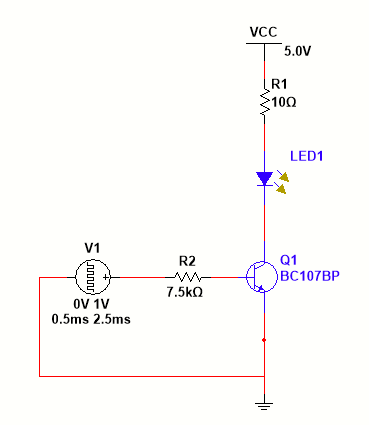
\includegraphics{Rapport/BallDispenser/BallCountSensor/graphics/Opstilling1.png}
    \caption{Opstilling for at pulse med IR-LED}
    \label{fig:IRLEDpuls}
\end{figure}

Næst designes fotodiode kredsløbet. Her bruges 4 komponenter: En modstand, en sample-hold kredsløb, en ADC-konverter og en PWM generator. Ideen er at bruge en modstanden til at forstærke en strøm signal om til en spænding, som så kan samples af sample-hold kredsløbet. ADC-konverteren oversætter vores spændingsværdi til et tal som kan bruges.
Vi benytter at $U=R\cdot I$, det betyder at hvis vi gerne vil detektere en lille strøm i form af en spænding, så har vi brug for en stor modstand. Derfor bruges der en $1M\Omega$ modstand. Et andet mulighed, var at bruge en transimpedans operatinsforstærker, som bruges i afsnit \fullref{hwdesign:sec:CupSensor} i dokumentet \textbf{Hardware Design}. Opstillingen for fotodioden er meget enkelt og kan ses på figur \ref{fig:fotodiode_opstilling}.
\begin{figure}[H]
    \centering
    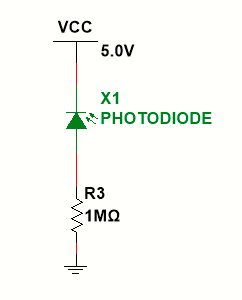
\includegraphics{Rapport/BallDispenser/BallCountSensor/graphics/Opstilling1_2.png}
    \caption{Opstilling for fotodiode}
    \label{fig:fotodiode_opstilling}
\end{figure}
På grund af et puls signal med IR-LED, vil der være en varians i spændingen over modstanden R3 i figur \ref{fig:fotodiode_opstilling}. Der ønskes en konstant spænding fordi det er nemmere at arbejde med, og fordi spænding skal være et udtryk for hvormange bolde der. Det er her sample-hold komponenten i PSoC er nyttigt. Som navnet siger, så samples der en spænding på et givet tidspunkt, og denne spænding holdes, indtil næste sampling. Der skal være styr på at timingen mellem IR-LED pulse og samplingerne er optimalt, sådan at vi har en dc-spænding ud af samplehold kredsløbet. Det er klart at både IR-LED transistor i figur 1.1 og samplehold komponenten skal drives af samme clock, så de er synkroniseret. Opstilling kan ses på  figur \ref{fig:PSoC_TopDesign}.
\begin{figure}[H]
    \centering
    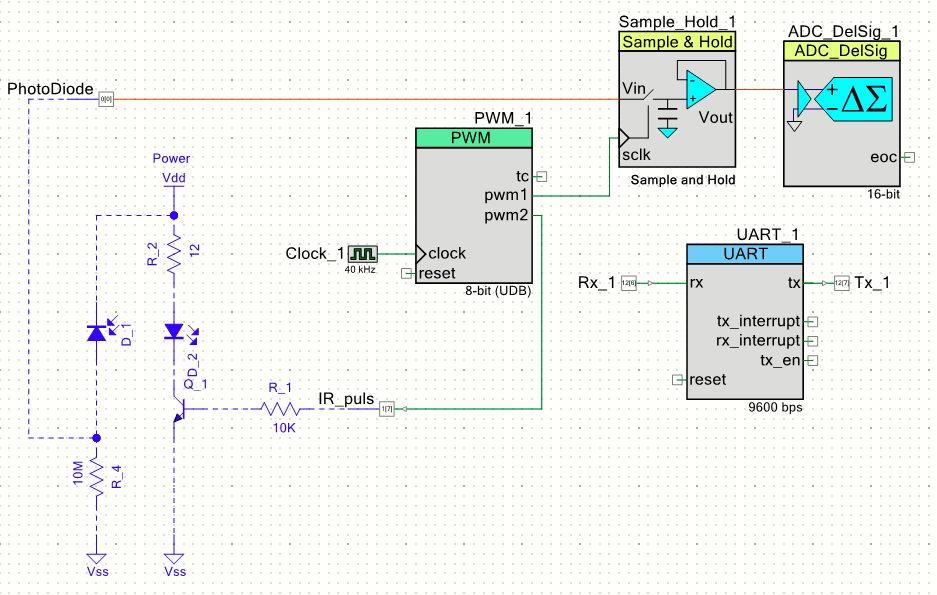
\includegraphics[width=1\textwidth]{Rapport/BallDispenser/BallCountSensor/graphics/Opstilling2.png}
    \caption{Opstilling for Ball Count sensor kredsløb}
    \label{fig:PSoC_TopDesign}
\end{figure}

\paragraph{Målinger og kalibrering}
\newline
\newline
Før kredsløbet implementeres sammen med PSoC er det en god ide at lave nogle målinger af vores IR-LED strøm og fotodiode spænding. Her laves kredsløbene fra figur figur \ref{fig:IRLEDpuls} og \ref{fig:fotodiode_opstilling} på fumlebræt og Analog Discovery og en power-supply fra lab bruges i stedet for PSoC til at drive og måle på kredsløbet. Først måles spændingen generet af fotodiodens reverse-biased strøm. Spændingen måles mellem modstanden R3 og fotodioden (figur \ref{fig:fotodiode_opstilling}). Ved alle målinger pulser vi med 400Hz med en pulsebredde på 20\% som beregnet tidligere i afsnittet.
\begin{figure}[H]
    \centering
    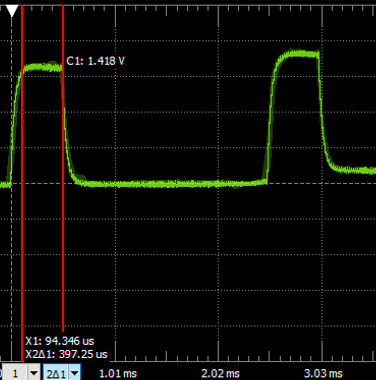
\includegraphics{Rapport/BallDispenser/BallCountSensor/graphics/Maling1.png}
    \caption{Måling af spændings rise-time ved fotodiodens modstand}
    \label{fig:Måling1_AD}
\end{figure}
På målingen i figur \ref{fig:Måling1_AD} kan man se, at spændingen genereret af fotodiodens strøm gennem en stor modstand, efterligner den pulse-signal som IR-LED drives med. Det vil sige ideen for hele sensoren er bekræftet. Det observeres også, at spændingen forårsaget af fotostrømmen afspejler IR-LED's signal pulsbredde og frekvens, men med en højere rising-time. Derfor ændres valget om at sample og pulse samtidigt. Målingen viser et dc-niveau i en pulsebredde med en tid på $397\mu s$ og en frekvens på 400Hz. Derfor må det antages at sensoren kan ses som et PWM signal på 400Hz med en pulsbredde på 15.9\%. Det beregnes således.
$$400Hz\cdot 397\mu s=0.159\%$$
For at være på den sikre side vælges der at sample med 400 Hz og en pulsbredde på 14\%. Kalibrering på PSoC kan ses på figur \ref{fig:PWM_timing}.
\begin{figure}[H]
    \centering
    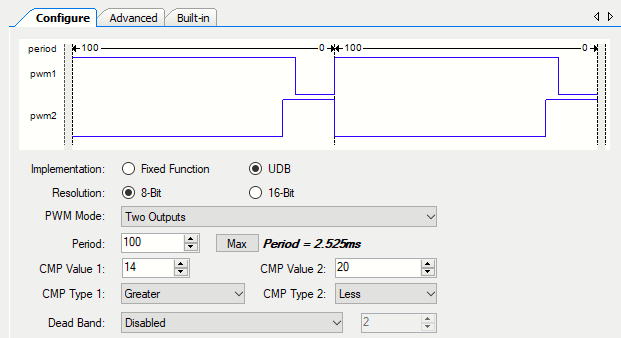
\includegraphics[width=1\textwidth]{Rapport/BallDispenser/BallCountSensor/graphics/PWM_timing.png}
    \caption{PWM signal pulsbredde timing}
    \label{fig:PWM_timing}
\end{figure}
Der gøres opmærksom på at Sample-Hold komponenten i PSoC sampler ved falling-edge. Næst måles strømmen gennem IR-LED, ved at måle spændingsfaldet over formodstanden R1 fra opstillingen i figur \ref{fig:IRLEDpuls}.
\begin{figure}[H]
    \centering
    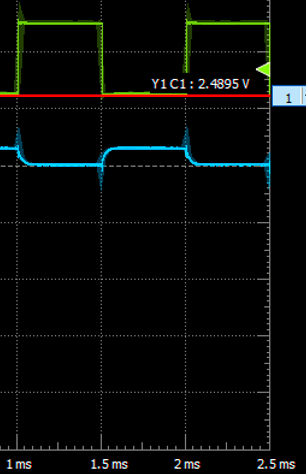
\includegraphics[width=0.27\textwidth]{Rapport/BallDispenser/BallCountSensor/graphics/Maling2.png}
    \caption{Måling af strøm gennem IR-LED}
    \label{fig:Måling2_AD}
\end{figure}
Her bergnes strømmen til 
$$\frac{(5-2.49)V}{10\Omega}=251mA$$
Her kalibreres ved at ændre på modstanden, så strømmen er lidt højere. Der vælges en modstand på $8.2\Omega$ som giver os en strøm på 306mA.
Kredsløbet er klar til at sættes sammen med PSoC. Opstillingen forbliver den samme som på figur \ref{fig:PSoC_TopDesign}. Hvor R2 er ændret til $8\Omega$ og R1 til $7.5k\Omega$
Ind i koden for PSoC bruges UART og ADC til at måle værdier alt efter hvormange bolde der i cylingerbeholderen. Hvor efter der kodes grænseværdier ind for antallet af bolde.

En tabel over de forskellige grænseværdier kan ses på tabel \ref{table:Treshold_BallCount}
\begin{table}[H]
\centering
\begin{tabular}{|C{0.1\textwidth}|C{0.25\textwidth}|L{0.25\textwidth}|}
\hline 
\textbf{Antal bolde} & \textbf{ADC værdi} & \textbf{status LED's}\\
\hline
1 & 1000 til 14999 & Rød\\
\hline
2 & 15000 til 29999 & Rød\\
\hline
3 & 30000 til 40000 & Slukket\\
\hline
4 & 1 til 400 & Grøn\\
\hline
\end{tabular}
\caption{Grænseværdier for BallCountSensor}
\label{table:Treshold_BallCount}
\end{table}
\end{document}